\documentclass[a4paper,10pt]{article}

\usepackage[margin=2.2cm]{geometry}
\usepackage[T1]{fontenc}
\usepackage{newtxtext,newtxmath}
\usepackage{graphicx}
\usepackage{booktabs}
\usepackage{tabularx}
\usepackage{longtable}
\usepackage{array}
\usepackage[section]{placeins}
\usepackage[hidelinks]{hyperref}

\graphicspath{{figures/huber_diagnostics/}{figures/story_slides/}{figures/decay_dynamics/}{figures/paper/}{results/analysis/oversmoothing_hooks_mp/}{results/analysis/oversmoothing_hooks_hzw/}}
\newcolumntype{Y}{>{\raggedright\arraybackslash}X}
\renewcommand{\arraystretch}{1.10}
\renewcommand{\thesection}{S\arabic{section}}
\renewcommand{\thetable}{S\arabic{table}}
\renewcommand{\thefigure}{S\arabic{figure}}

\title{\bfseries Supplementary Information\\Robust Global Virtual-Node Graph Neural Networks for Crystal Band-Gap Prediction with Cross-Source Label Consistency Analysis}
\author{Jiarui Liu\textsuperscript{1}, Junjie Liu\textsuperscript{1,*}, and Shunbo Hu\textsuperscript{1,*}}
\date{July 2026}

\begin{document}
\maketitle

\section{Structure-first MP--HZW data audit figure}
\label{sec:si-data-audit}

Panel (a) reports the audit conflict statistics under the audit thresholds (metal-like \(\le 0.05\ \mathrm{eV}\) or a metallic flag; non-metal \(\ge 0.10\ \mathrm{eV}\); same-class numerical disagreement \(>1\ \mathrm{eV}\)); the corresponding counts are tabulated as Table~1 of the main text. Panel (b) is the actual T-series filtering waterfall under the stricter export zero-gap threshold (\(\le 10^{-6}\ \mathrm{eV}\)), ending at the 84,550 equal-atom structures whose identical split is evaluated with both MP and HZW labels. The two panels use different, purpose-specific thresholds and are self-contained; they must not be combined row-wise.

\begin{figure}[htbp]
\centering
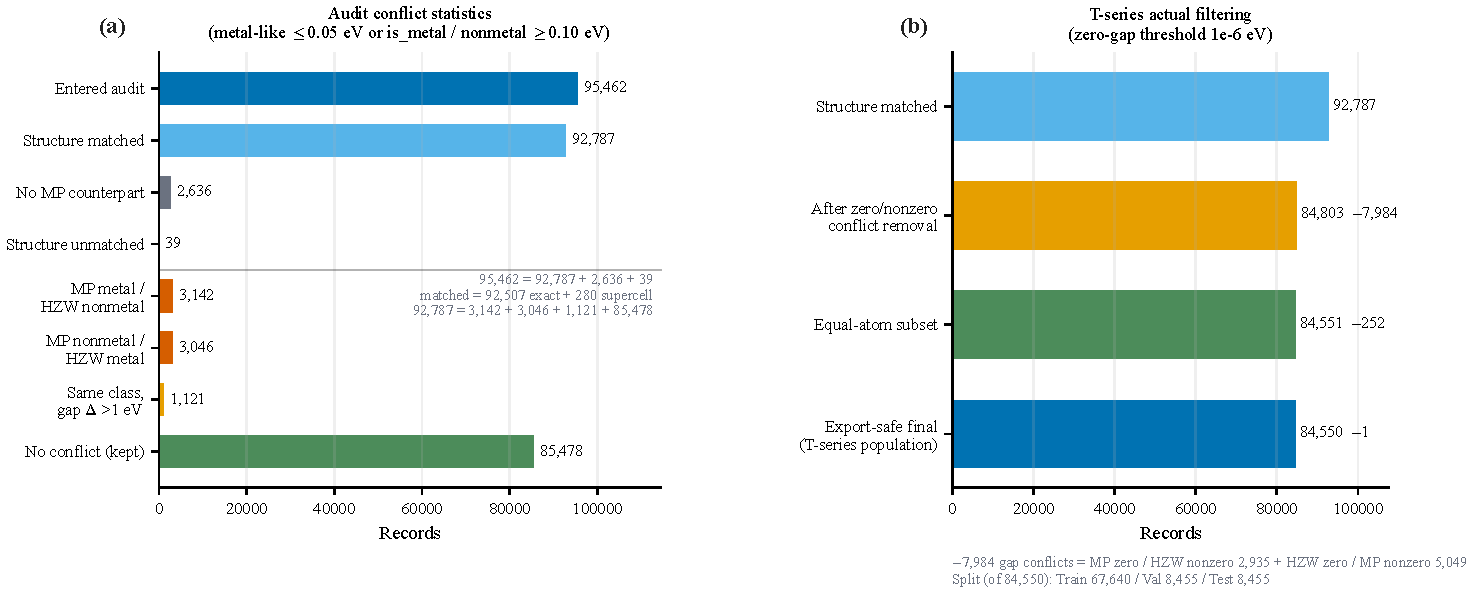
\includegraphics[width=\textwidth]{fig2_data_audit.pdf}
\caption{Structure-first data construction, shown as two self-contained ledgers. (a) Audit conflict statistics under the audit thresholds. (b) The T-series filtering waterfall, ending at 84,550 structures.}
\label{fig:si-data-audit}
\end{figure}

\section{Absolute per-element error map}
\label{sec:si-element-mae}

This map reports the absolute per-element test error of the robust model and complements the baseline-to-robust change map of the main text, which carries the evidence that the virtual-node and Huber gains are chemically broad. As in the main text, a structure containing element \(X\) contributes its absolute error to \(X\); elements with fewer than 30 test structures are grayed, and elements absent from the test split are left white.

\begin{figure}[htbp]
\centering
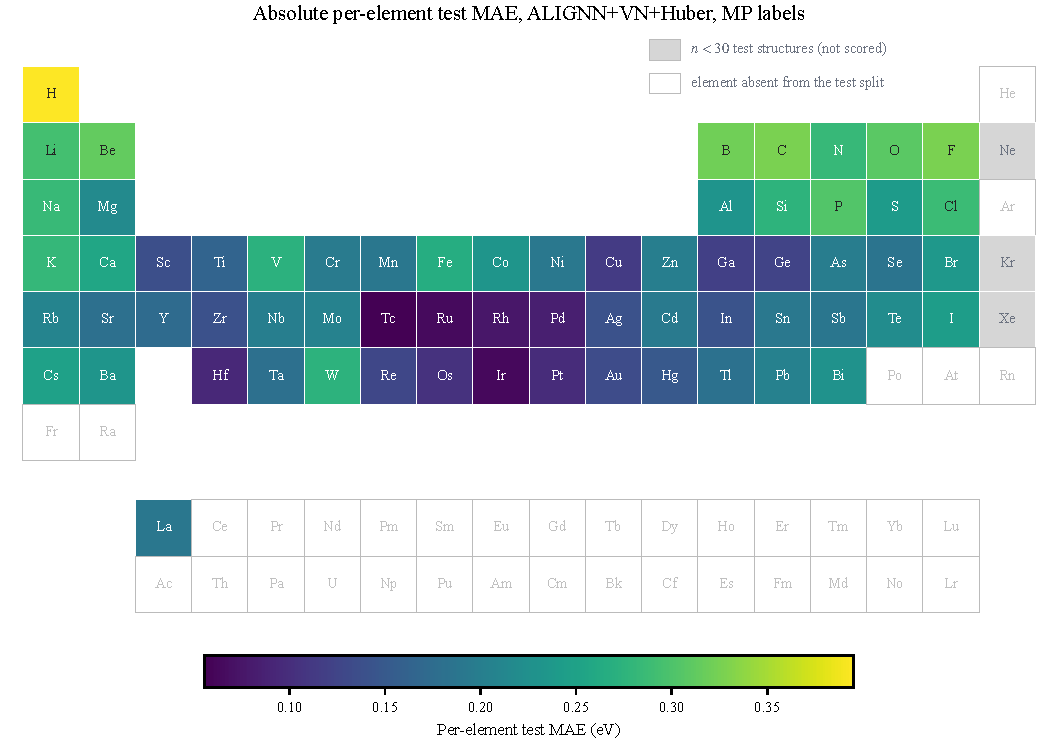
\includegraphics[width=0.9\textwidth]{figS5_element_mae_absolute.pdf}
\caption{Absolute per-element test MAE of the robust model (T7, ALIGNN + virtual node + Huber) on MP labels, seed-42 run, over the periodic table.}
\label{fig:si-element-mae}
\end{figure}

\section{Exploratory HZW experiments}

The E-series used an earlier HZW data stage and is reported only to document the design lineage. These values are not directly compared with the final matched T-series.

\begin{table}[htbp]
\centering
\caption{Selected early HZW experimental results.}
\label{tab:early-hzw}
\small
\begin{tabular}{l l r r r}
\toprule
ID & Model & MAE & RMSE & \(R^2\) \\
\midrule
E1 & CGCNN & 0.3022 & 0.5303 & 0.8847 \\
E2 & ALIGNN & 0.2314 & 0.4713 & 0.9089 \\
E4 & ALIGNN + virtual node & 0.2201 & 0.4746 & 0.9077 \\
E6 & Physics-constrained ALIGNN & 0.2212 & 0.4539 & 0.9155 \\
E8 & Two attentive virtual nodes & 0.2285 & 0.4945 & 0.8997 \\
E12 & Size-supervised dual slot & 0.2179 & 0.4712 & 0.9090 \\
E13 & E12 + valid-mask physics loss & 0.2119 & 0.4616 & 0.9126 \\
\bottomrule
\end{tabular}
\end{table}

\section{Size-dependent dual-node diagnostic}

\begin{table}[htbp]
\centering
\caption{Strict-clean MP-label comparison of a single (run S4) and a dual (run S13) plain virtual node. S4 and S13 are S-series run identifiers (Section~S10), not supplementary table numbers.}
\label{tab:size-buckets}
\small
\begin{tabular}{l r r r r l}
\toprule
Atom bucket & \(n\) & Mean atoms & S4 MAE & S13 MAE & Winner \\
\midrule
\(\le 10\) & 2,327 & 6.003 & 0.118300 & 0.118845 & S4 \\
11--20 & 1,873 & 15.601 & 0.175596 & 0.172570 & S13 \\
21--40 & 2,106 & 29.986 & 0.235496 & 0.243521 & S4 \\
41--80 & 1,452 & 57.574 & 0.279100 & 0.280506 & S4 \\
81--160 & 369 & 106.488 & 0.321578 & 0.307066 & S13 \\
\(>160\) & 27 & 190.333 & 0.278618 & 0.266599 & S13 \\
\midrule
Overall & 8,154 & -- & \textbf{0.200094} & 0.201181 & S4 \\
\(>80\) merged & 396 & 112.205 & 0.318649 & \textbf{0.304307} & S13 \\
\bottomrule
\end{tabular}
\end{table}

\section{Complete final T-series metrics}

\begin{table}[htbp]
\centering
\caption{Complete T-series metrics and resource accounting. Values are from the original seed-42 runs; multi-seed replication is reported in Table~\ref{tab:multiseed}.}
\label{tab:full-t-series}
\scriptsize
\begin{tabular}{l l r r r r r r}
\toprule
Source & ID & MAE & RMSE & \(R^2\) & F1 & Epoch & GPU GB \\
\midrule
MP & T1 & 0.366338 & 0.612696 & 0.858769 & 0.788246 & 49 & 2.992 \\
MP & T2 & 0.240043 & 0.490694 & 0.909414 & 0.882637 & 50 & 10.164 \\
MP & T3 & 0.285903 & 0.584315 & 0.871550 & 0.889726 & 41 & 2.486 \\
MP & T4 & 0.232520 & 0.505610 & 0.903823 & 0.909240 & 49 & 10.312 \\
MP & T6 & 0.229585 & 0.512560 & 0.901161 & 0.913312 & 46 & 10.174 \\
MP & T7 & 0.224931 & 0.503546 & 0.904607 & 0.911331 & 49 & 10.312 \\
MP & T8 & 0.230402 & 0.496074 & 0.907417 & 0.905809 & 50 & 10.174 \\
MP & T9 & 0.226028 & 0.495817 & 0.907513 & 0.914071 & 50 & 10.175 \\
MP & T10 & 0.223686 & 0.497333 & 0.906946 & 0.915455 & 47 & 10.313 \\
\midrule
HZW & T1 & 0.338152 & 0.565454 & 0.878497 & 0.788237 & 49 & 2.992 \\
HZW & T2 & 0.212124 & 0.436147 & 0.927713 & 0.890299 & 50 & 10.164 \\
HZW & T3 & 0.256572 & 0.535916 & 0.890859 & 0.892629 & 43 & 2.486 \\
HZW & T4 & 0.201762 & 0.448621 & 0.923519 & 0.909613 & 49 & 10.312 \\
HZW & T6 & 0.198584 & 0.447143 & 0.924022 & 0.913786 & 46 & 10.174 \\
HZW & T7 & 0.194002 & 0.445837 & 0.924465 & 0.915401 & 49 & 10.312 \\
HZW & T8 & 0.202603 & 0.448503 & 0.923559 & 0.909881 & 50 & 10.174 \\
HZW & T9 & 0.197707 & 0.448776 & 0.923466 & 0.916846 & 46 & 10.175 \\
HZW & T10 & 0.197034 & 0.453592 & 0.921815 & 0.913209 & 45 & 10.313 \\
\bottomrule
\end{tabular}
\end{table}

\section{Broadcast-decay residual diagnostics}

\begin{table}[htbp]
\centering
\caption{Overall T7 versus T10 residual diagnostics. Bias is mean prediction residual \(\hat y-y\).}
\label{tab:decay-residuals}
\scriptsize
\begin{tabular}{l l r r r r r r}
\toprule
Source & Model & MAE & RMSE & Bias & Median AE & P90 AE & \(>1\) eV ratio \\
\midrule
MP & T7 Huber & 0.224931 & 0.503546 & 0.025437 & 0.066248 & 0.582403 & 0.041514 \\
MP & T10 decay + Huber & 0.223686 & 0.497333 & 0.013963 & 0.064191 & 0.588758 & 0.041632 \\
HZW & T7 Huber & 0.194002 & 0.445837 & 0.025182 & 0.059381 & 0.498598 & 0.029568 \\
HZW & T10 decay + Huber & 0.197034 & 0.453592 & 0.010850 & 0.060386 & 0.507704 & 0.030751 \\
\bottomrule
\end{tabular}
\end{table}

\section{Residual and bucket-level diagnostics}

The per-epoch training and validation curves of the six core models are shown as Figure~2 of the main text; the observations drawn from them are discussed there. This section collects the remaining optimization diagnostics. Figure~\ref{fig:optimization} gives the robust-loss residual diagnostics behind the T4/T7 comparison, and Figure~\ref{fig:decay-buckets} shows the bucket-level MAE change when broadcast decay is added on top of the Huber recipe (T10 versus T7).

\begin{figure}[htbp]
\centering
\begin{minipage}[t]{0.49\textwidth}
\textbf{(a)}\par\smallskip
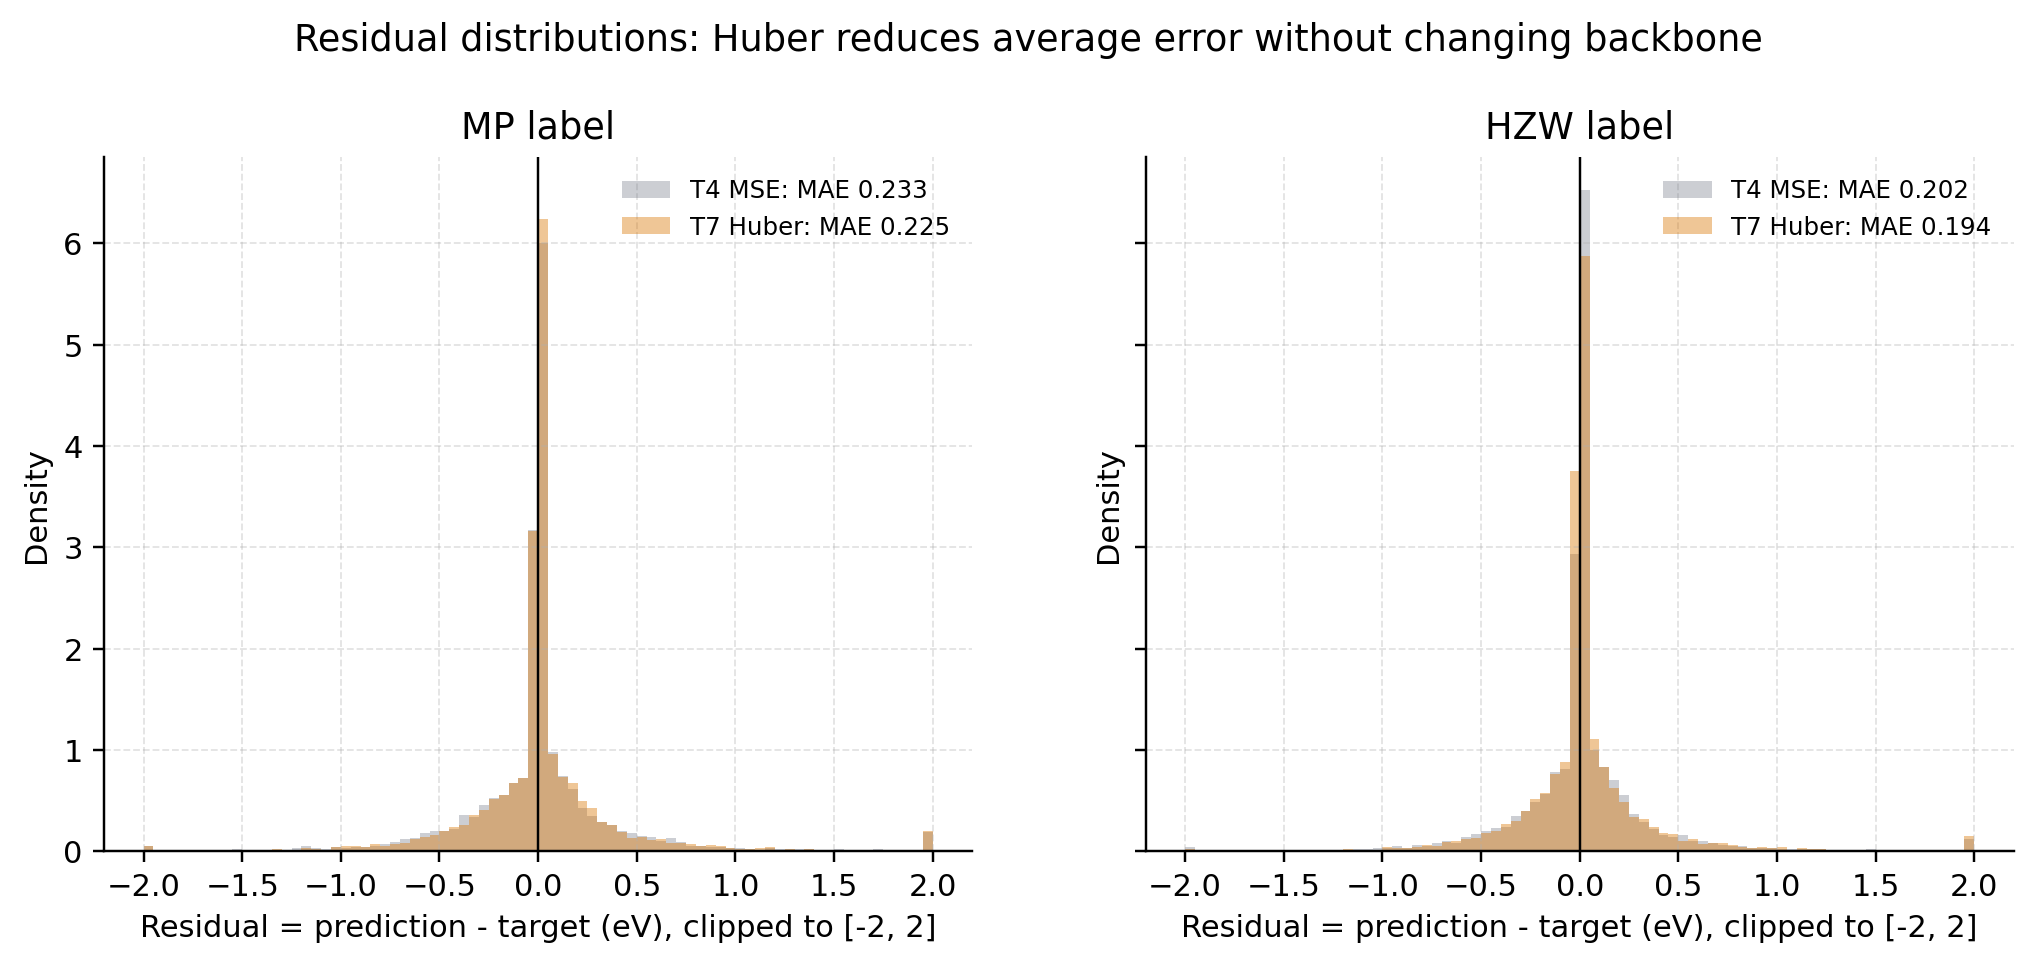
\includegraphics[width=\linewidth]{residual_hist_t4_vs_t7.png}
\end{minipage}
\hfill
\begin{minipage}[t]{0.49\textwidth}
\textbf{(b)}\par\smallskip
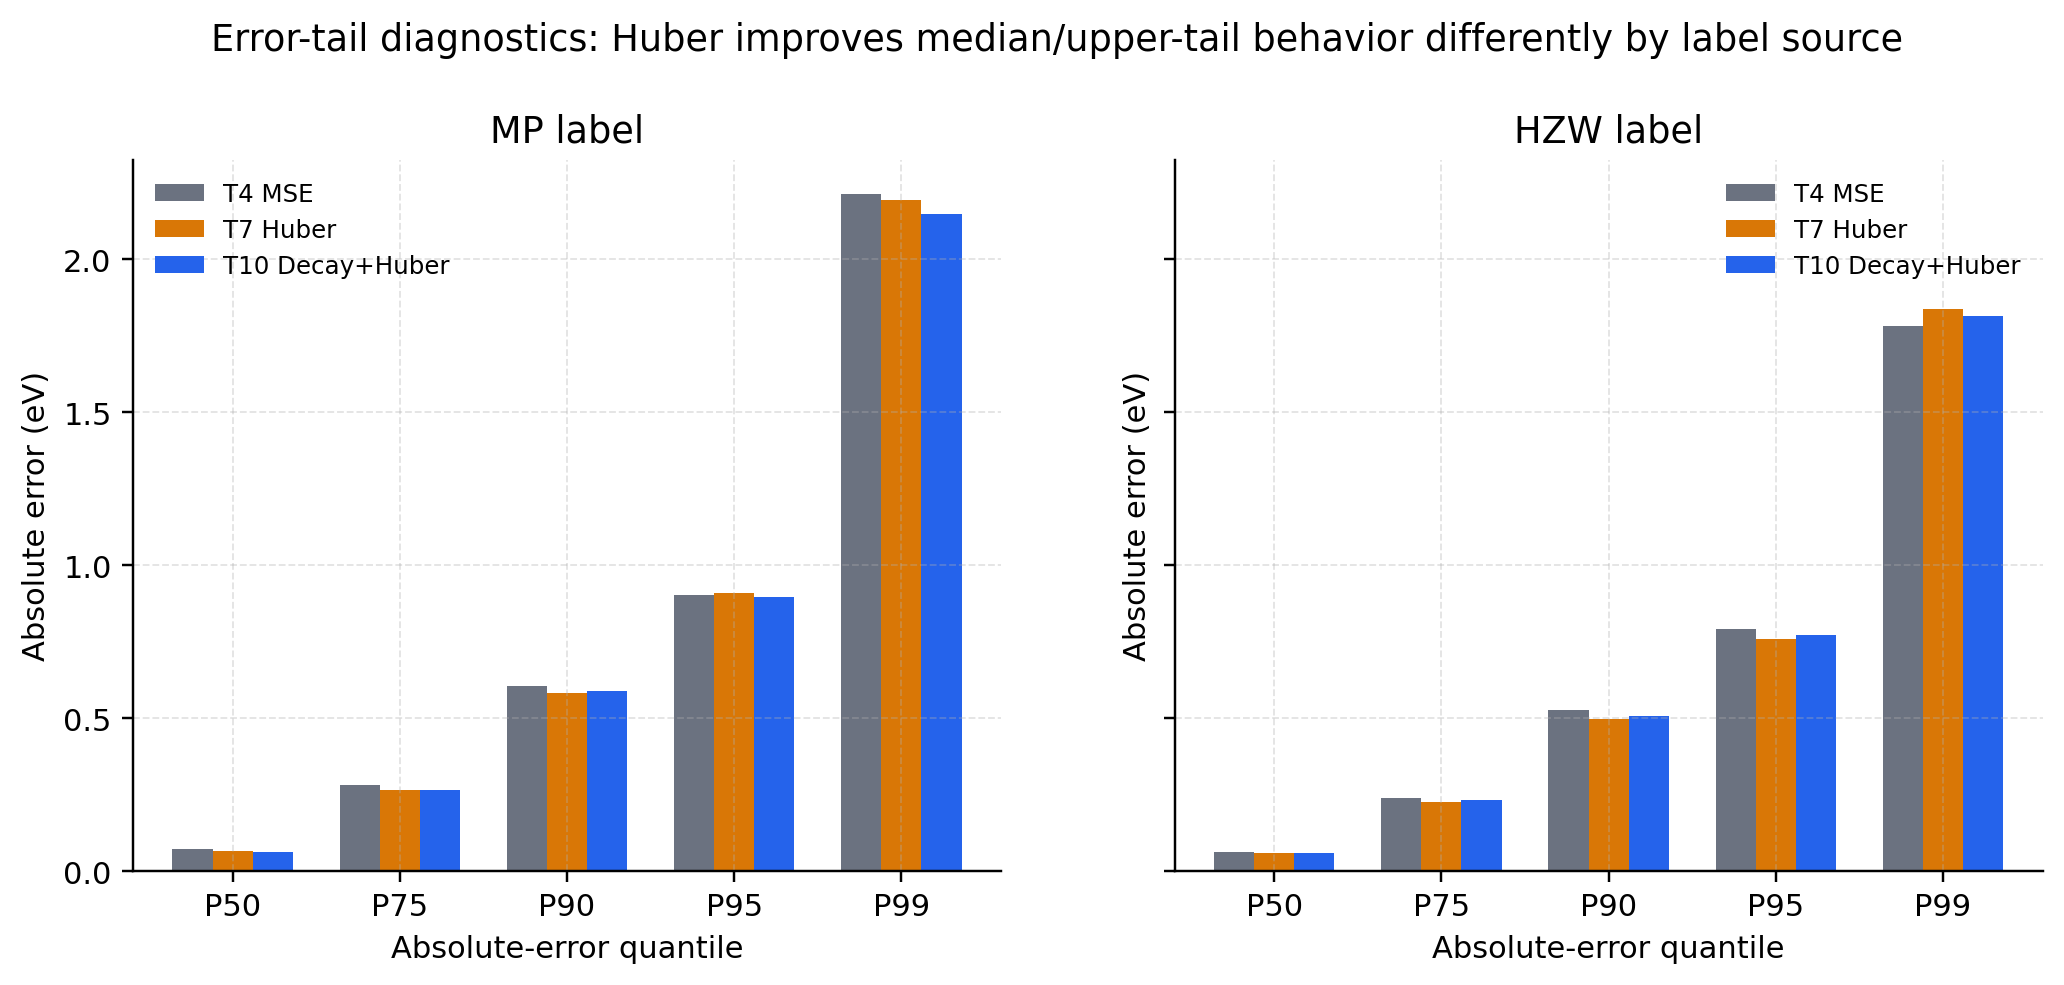
\includegraphics[width=\linewidth]{abs_error_quantiles_t4_t7_t10.png}
\end{minipage}
\caption{Robust-loss residual diagnostics. (a) Prediction-residual histograms for the MSE-trained (T4) and Huber-trained (T7) virtual-node models. (b) Absolute-error quantiles for T4, T7, and T10.}
\label{fig:optimization}
\end{figure}

\begin{figure}[htbp]
\centering
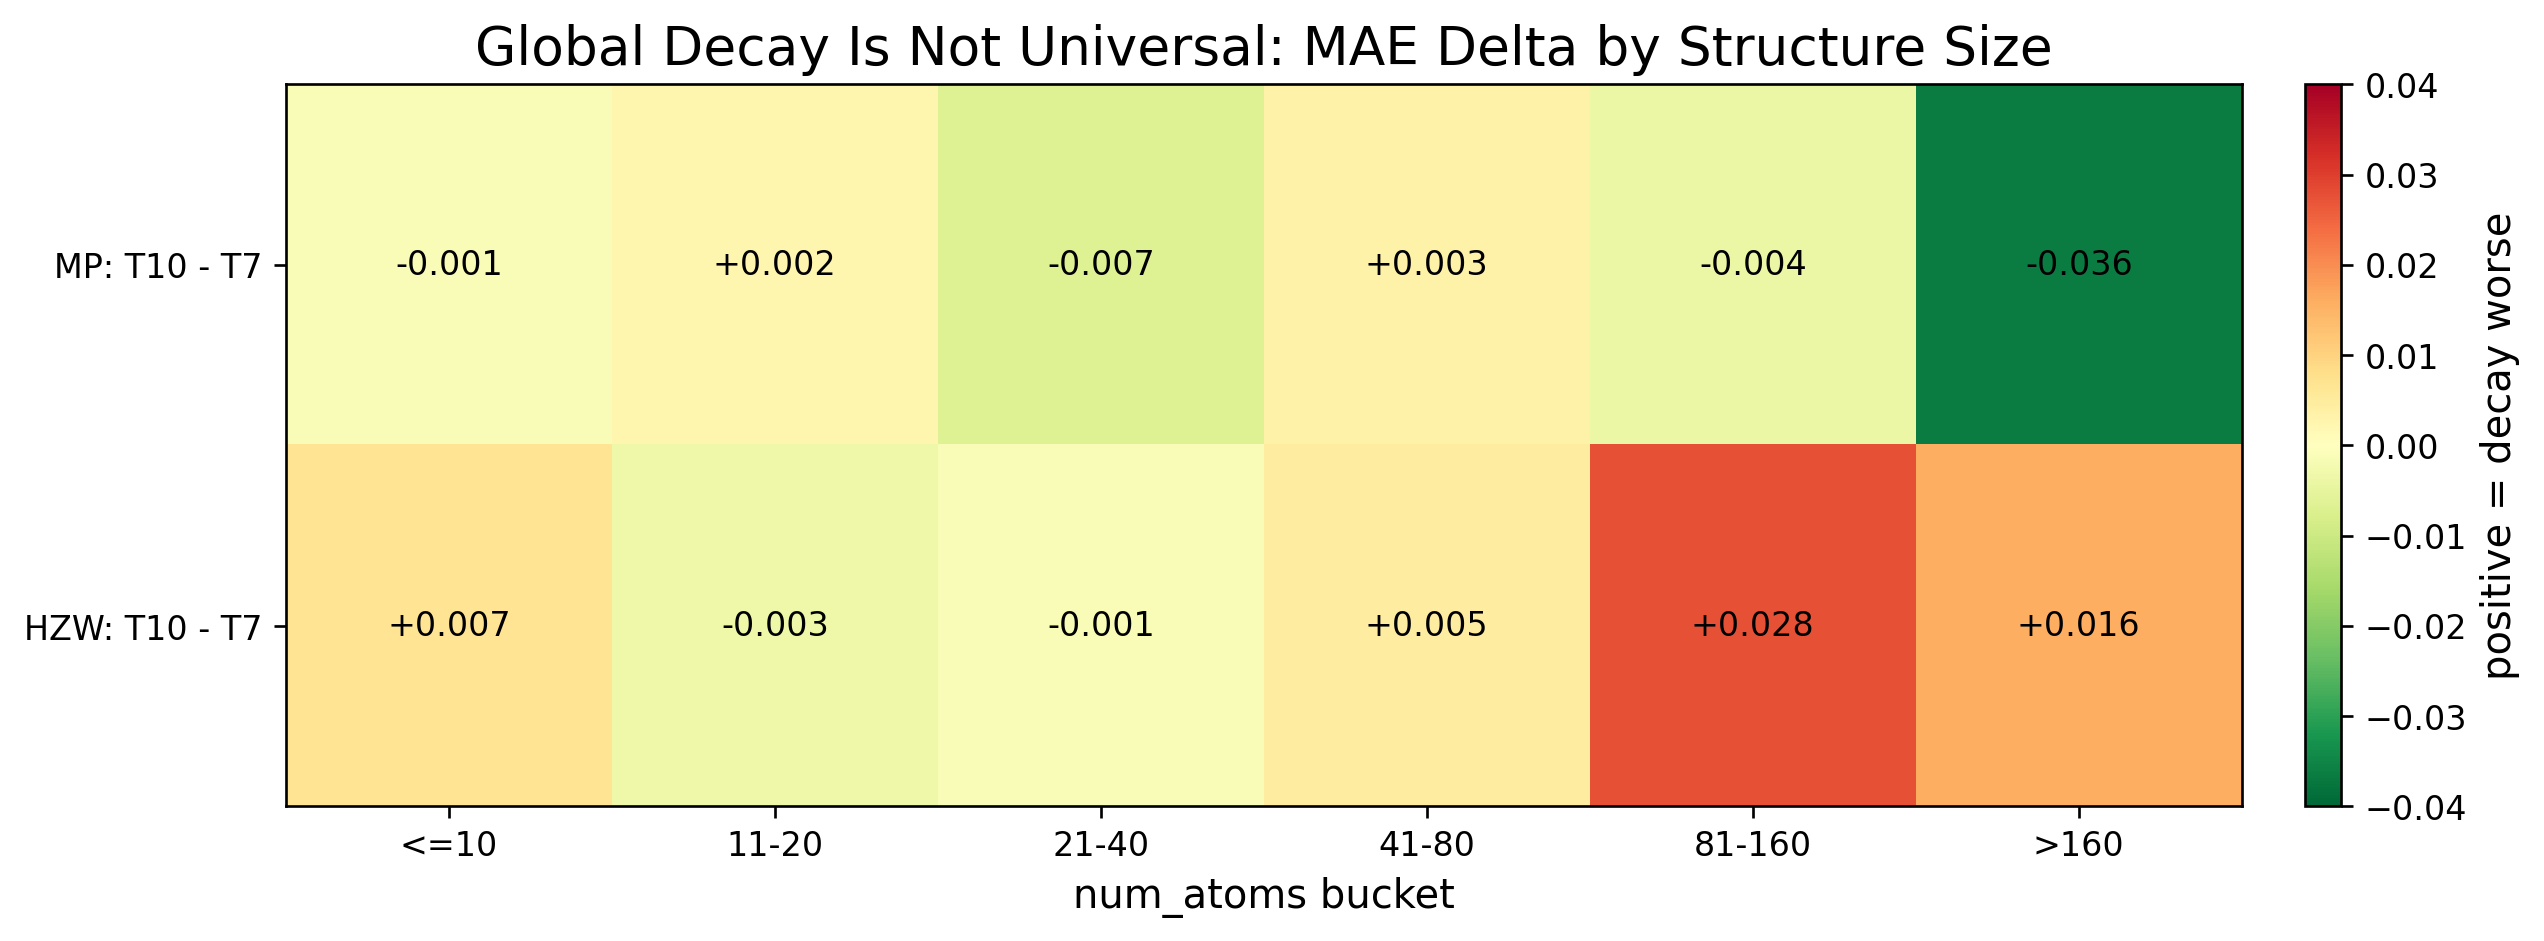
\includegraphics[width=0.82\textwidth]{decay_delta_heatmap.png}
\caption{Bucket-level T10--T7 MAE changes. Negative values indicate improvement from broadcast decay.}
\label{fig:decay-buckets}
\end{figure}

\section{Layer-wise representation diagnostics}

Figure~\ref{fig:layerwise-cosine} reports the hook-based layer-wise representation diagnostic for the recommended checkpoints on both label sources.

\begin{figure}[htbp]
\centering
\begin{minipage}[t]{0.49\textwidth}
\textbf{(a) MP}\par\smallskip
\includegraphics[width=\linewidth]{results/analysis/oversmoothing_hooks_mp/layerwise_mean_pairwise_cosine.png}
\end{minipage}
\hfill
\begin{minipage}[t]{0.49\textwidth}
\textbf{(b) HZW}\par\smallskip
\includegraphics[width=\linewidth]{results/analysis/oversmoothing_hooks_hzw/layerwise_mean_pairwise_cosine.png}
\end{minipage}
\caption{Layer-wise mean pairwise cosine similarity from the hook-based checkpoint diagnostic.}
\label{fig:layerwise-cosine}
\end{figure}

\section{E-series model lineage}

Table~\ref{tab:e-lineage} lists the complete E1--E13 design lineage of the exploratory HZW stage summarized in Section~S3; as noted there, the E-series used an earlier data stage and is not directly comparable to the final T-series.

\begin{table}[htbp]
\centering
\caption{Complete E-series design lineage.}
\label{tab:e-lineage}
\scriptsize
\begin{tabularx}{\textwidth}{p{1.1cm} p{3.5cm} Y}
\toprule
ID & Model & Main idea \\
\midrule
E1 & CGCNN & Crystal graph convolution baseline. \\
E2 & ALIGNN & Atom graph plus line graph for bond-angle modeling. \\
E3 & M3GNet & Many-body material graph baseline. \\
E4 & ALIGNN + plain virtual node & Single low-cost graph-level context channel. \\
E5 & ALIGNN + Transformer & Full global attention after ALIGNN encoding. \\
E6 & Physics constraint & CBM/VBM auxiliary supervision with a validity mask. \\
E7 & One attentive virtual node & Single attention-based global slot. \\
E8 & Two attentive virtual nodes & Dual global slots with slot interaction. \\
E9/E10 & Size-aware gates & Explicit second-slot activation conditioned on size. \\
E11 & Routed ensemble & Validation-selected routing between single and dual models. \\
E12 & Size-supervised dual slot & Atom count supervises, but does not directly enter, the gate. \\
E13 & E12 + physics & Size-supervised dual slot plus valid-mask physics loss. \\
\bottomrule
\end{tabularx}
\end{table}

\section{Series nomenclature}

Models are indexed by a letter-and-number code that records the experimental stage at which they were run. The \textbf{T series} denotes the final matched-benchmark stage: models trained on the relaxed-clean equal-atom MP--HZW matched dataset that underlies all main-text results. The \textbf{E series} denotes the exploratory HZW stage on an earlier data snapshot (Tables~\ref{tab:early-hzw} and~\ref{tab:e-lineage}); E-series numbers document design lineage only and are not directly comparable with the T series. The \textbf{S series} denotes the strict-filter stage: models trained on the strictly label-consistent subset (\(\mathrm{MP\ is\_metal}=\mathrm{HZW\ is\_metal}\), \(|\Delta\mathrm{gap}|\le 0.5\) eV, and per-atom volume difference \(\le 8\%\); Table~\ref{tab:size-buckets}). Within each series the numeric index is an internal run identifier; throughout the main text these codes are replaced by descriptive names. The mapping for the three headline T-series models is given in Table~\ref{tab:series-map}.

\begin{table}[htbp]
\centering
\caption{Descriptive-name mapping for the headline T-series (final matched-benchmark stage) models.}
\label{tab:series-map}
\small
\begin{tabularx}{\textwidth}{l l Y}
\toprule
ID & Descriptive name & Definition \\
\midrule
T1 & CGCNN & Crystal graph convolutional baseline. \\
T2 & ALIGNN & ALIGNN baseline (atom graph plus line graph). \\
T3 & M3GNet & M3GNet baseline (trained from scratch). \\
T4 & ALIGNN+VN & ALIGNN with a single plain virtual node. \\
T7 & ALIGNN+VN+Huber & T4 with a Huber (smooth-L1, \(\beta=0.5\)) final-gap loss. \\
T10 & ALIGNN+VN+Huber+decay & T7 with a broadcast-decay schedule (epochs 10\(\to\)50, minimum scale 0.25). \\
\bottomrule
\end{tabularx}
\end{table}

\section{Paired bootstrap significance of MAE differences}

\begin{table}[htbp]
\centering
\caption{Paired bootstrap of test-set MAE differences (\(B=10{,}000\), bootstrap seed 20260714), computed on identical resampled test samples. \(\Delta\mathrm{MAE}=\mathrm{MAE}(a)-\mathrm{MAE}(b)\); a negative value favors the first model. \(P(\Delta<0)\) is the bootstrap probability that the first model has lower MAE. Data source: \textnormal{results/analysis/paired\_bootstrap.csv}.}
\label{tab:paired-bootstrap}
\small
\begin{tabular}{l l r c r c}
\toprule
Source & Pair & \(\Delta\)MAE (eV) & 95\% CI & \(P(\Delta<0)\) & Sig.\ 95\% \\
\midrule
MP  & T4\(-\)T2  & \(-0.0075\) & \([-0.0121,\,-0.0028]\) & 0.9995 & yes \\
MP  & T7\(-\)T4  & \(-0.0076\) & \([-0.0122,\,-0.0029]\) & 0.9994 & yes \\
MP  & T7\(-\)T2  & \(-0.0151\) & \([-0.0198,\,-0.0103]\) & 1.0000 & yes \\
MP  & T10\(-\)T7 & \(-0.0012\) & \([-0.0058,\,+0.0033]\) & 0.7022 & no \\
MP  & T10\(-\)T4 & \(-0.0088\) & \([-0.0135,\,-0.0043]\) & 0.9999 & yes \\
\midrule
HZW & T4\(-\)T2  & \(-0.0104\) & \([-0.0147,\,-0.0060]\) & 1.0000 & yes \\
HZW & T7\(-\)T4  & \(-0.0078\) & \([-0.0120,\,-0.0035]\) & 0.9997 & yes \\
HZW & T7\(-\)T2  & \(-0.0181\) & \([-0.0224,\,-0.0138]\) & 1.0000 & yes \\
HZW & T10\(-\)T7 & \(+0.0030\) & \([-0.0011,\,+0.0071]\) & 0.0706 & no \\
HZW & T10\(-\)T4 & \(-0.0047\) & \([-0.0094,\,-0.0001]\) & 0.9780 & yes \\
\bottomrule
\end{tabular}
\end{table}

All five model pairs are reported on both label sources. The virtual-node gain (T4\(-\)T2) and the Huber gain (T7\(-\)T4) are each significant on both label sources, as is the combined gain (T7\(-\)T2: \(-0.0151\) eV on MP, \(-0.0181\) eV on HZW), whereas the decay effect (T10\(-\)T7) is not statistically resolved on either label source, with opposite signs in the seed-42 point estimates.

\section{Cross-label evaluation}

\begin{table}[htbp]
\centering
\caption{Cross-label evaluation: each model's predictions are scored against both the label source it was trained on and the other source, over the identical intersected test structures (\(n=8{,}455\)). Data source: \textnormal{results/analysis/cross\_label\_eval.csv}.}
\label{tab:cross-label}
\small
\begin{tabular}{l l l r r}
\toprule
Model & Train label & Eval label & MAE & RMSE \\
\midrule
ALIGNN (T2)                & MP  & MP  & 0.2400 & 0.4907 \\
ALIGNN (T2)                & MP  & HZW & 0.2479 & 0.4992 \\
ALIGNN (T2)                & HZW & MP  & 0.2453 & 0.4978 \\
ALIGNN (T2)                & HZW & HZW & 0.2121 & 0.4361 \\
\midrule
ALIGNN+VN (T4)             & MP  & MP  & 0.2325 & 0.5056 \\
ALIGNN+VN (T4)             & MP  & HZW & 0.2389 & 0.5092 \\
ALIGNN+VN (T4)             & HZW & MP  & 0.2364 & 0.5121 \\
ALIGNN+VN (T4)             & HZW & HZW & 0.2018 & 0.4486 \\
\midrule
ALIGNN+VN+Huber (T7)       & MP  & MP  & 0.2249 & 0.5035 \\
ALIGNN+VN+Huber (T7)       & MP  & HZW & 0.2314 & 0.5073 \\
ALIGNN+VN+Huber (T7)       & HZW & MP  & 0.2300 & 0.5132 \\
ALIGNN+VN+Huber (T7)       & HZW & HZW & 0.1940 & 0.4458 \\
\midrule
ALIGNN+VN+Huber+decay (T10) & MP  & MP  & 0.2237 & 0.4973 \\
ALIGNN+VN+Huber+decay (T10) & MP  & HZW & 0.2290 & 0.4974 \\
ALIGNN+VN+Huber+decay (T10) & HZW & MP  & 0.2325 & 0.5175 \\
ALIGNN+VN+Huber+decay (T10) & HZW & HZW & 0.1970 & 0.4536 \\
\bottomrule
\end{tabular}
\end{table}

For the seed-42 checkpoints, the sign of the estimated T10\(-\)T7 MAE difference follows the training-label source under both evaluation labels: models trained on MP have T10 MAE at or below T7 under both evaluation labels (\(-0.0012\) eV vs.\ MP labels, \(-0.0024\) eV vs.\ HZW labels), while models trained on HZW have T10 MAE above T7 under both evaluation labels (\(+0.0025\) eV vs.\ MP labels, \(+0.0030\) eV vs.\ HZW labels). We computed a paired bootstrap (\(B=10{,}000\), bootstrap seed 20260714) for each of the four cross-label conditions, reusing the method of Table~\ref{tab:paired-bootstrap}; all four 95\% confidence intervals cross zero: MP-trained, MP eval \([-0.0058,\,+0.0033]\); MP-trained, HZW eval \([-0.0070,\,+0.0021]\); HZW-trained, MP eval \([-0.0015,\,+0.0066]\); HZW-trained, HZW eval \([-0.0011,\,+0.0071]\). All four comparisons are statistically unresolved. Their sign pattern suggests an association with the training-label source, but the comparisons reuse the same test structures and seed-42 checkpoints; they are not independent replications and do not establish a causal mechanism or seed-stable source dependence. All entries are seed-42 checkpoints. The ALIGNN baseline rows (T2) carry no decay comparison and are included for reference only.

\section{Broadcast-decay training dynamics}

\begin{figure}[htbp]
\centering
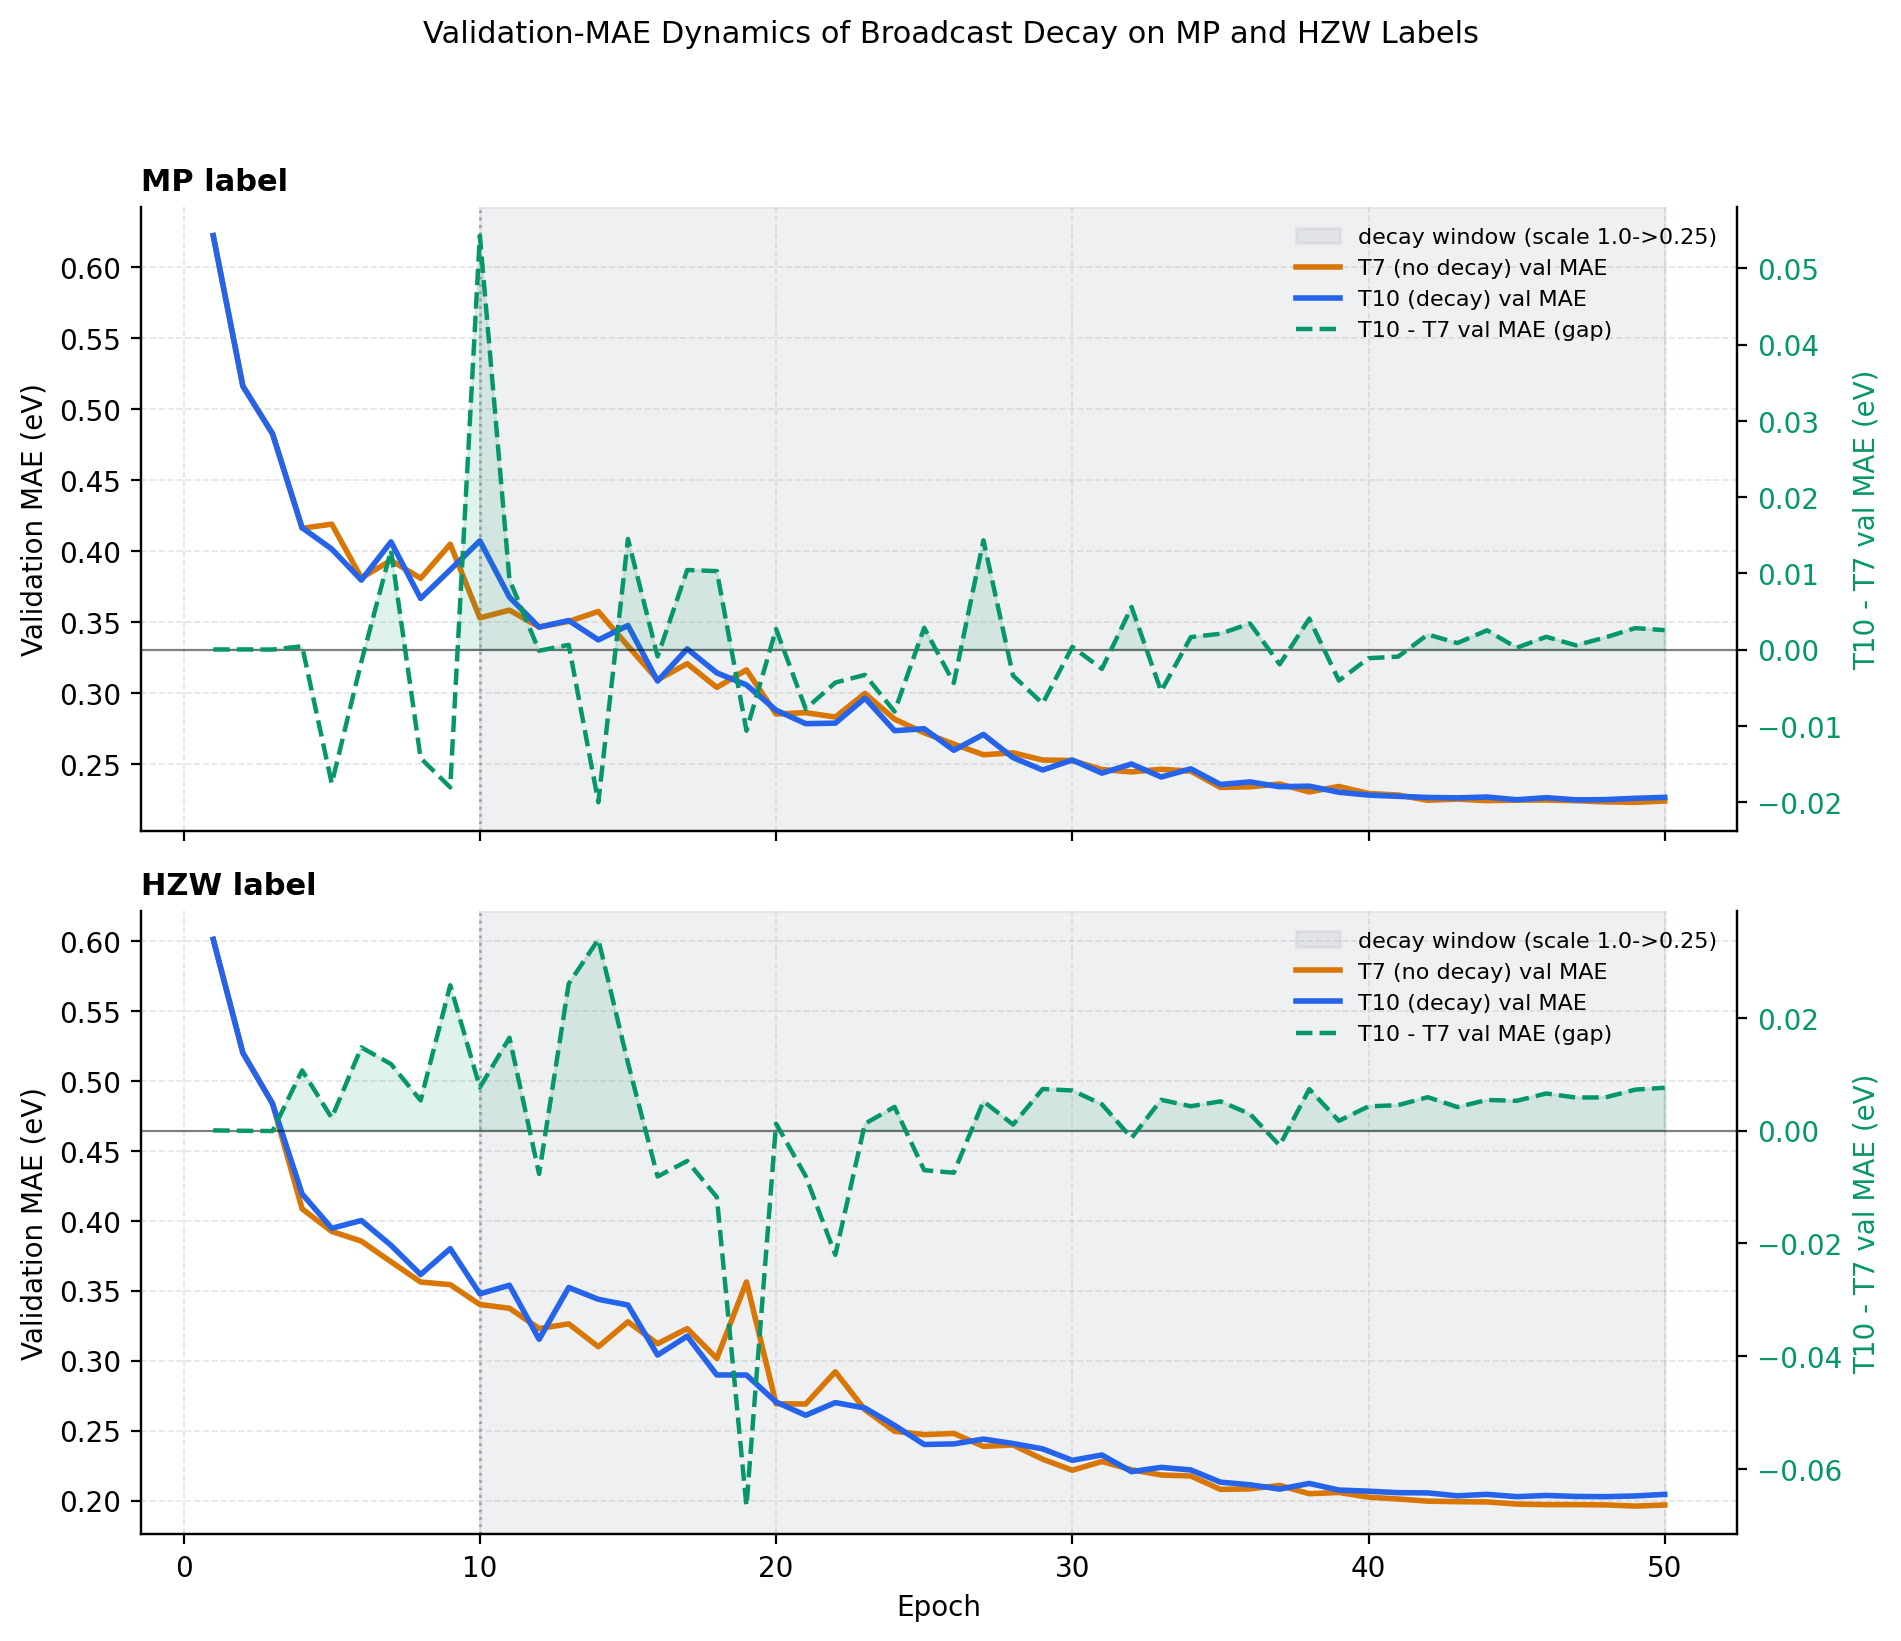
\includegraphics[width=0.82\textwidth]{decay_val_mae_dynamics.png}
\caption{Per-epoch validation-MAE dynamics for T7 (ALIGNN+VN+Huber) and T10 (ALIGNN+VN+Huber+decay) on both label sources, with the T10\(-\)T7 difference overlaid and the broadcast-decay window (epochs 10\(\to\)50) shaded. On HZW the T10\(-\)T7 difference stabilizes at a positive value (\(\sim\)+0.005--0.008 eV, i.e.\ T10 worse) through the deep-decay region and climbs further in the late epochs, whereas on MP the difference oscillates near zero.}
\label{fig:decay-dynamics}
\end{figure}

\section{Broadcast-decay cohort profiles}

\begin{table}[htbp]
\centering
\caption{Chemical, structural and label profiles of the decay-harmed vs.\ decay-benefited HZW cohorts (worst / best 10\% of per-sample \(\Delta\mathrm{AE}=\mathrm{AE}(\mathrm{T10})-\mathrm{AE}(\mathrm{T7})\); each cohort \(n\approx846\)). ``Diff'' is the harmed-minus-benefited difference in the fraction of samples in each category, in percentage points, with a bootstrap 95\% CI. Only dimensions whose CI excludes zero are marked significant. Data source: \textnormal{results/analysis/decay\_mechanism/decay\_cohorts\_profile.csv}.}
\label{tab:decay-cohorts}
\small
\begin{tabular}{l l r r r c c}
\toprule
Dimension & Category & Harmed \% & Benef.\ \% & Diff (pp) & 95\% CI (pp) & Sig. \\
\midrule
Element family  & transition metal        & 69.98 & 65.13 & \(+4.85\) & \([+0.12,\,+9.34]\) & yes \\
Crystal system  & tetragonal              &  6.97 &  9.81 & \(-2.84\) & \([-5.44,\,-0.12]\) & yes \\
Symmetry class  & medium (SG 75--167)     & 14.07 & 18.44 & \(-4.37\) & \([-8.04,\,-0.95]\) & yes \\
Target gap      & \((0,0.5)\) eV          &  9.10 & 12.29 & \(-3.19\) & \([-6.15,\,-0.12]\) & yes \\
\midrule
Element family  & halogen (control)       & 25.89 & 25.18 & \(+0.71\) & \([-3.55,\,+4.85]\) & no \\
Label           & MP metal (control)      & 15.25 & 18.09 & \(-2.84\) & \([-6.50,\,+0.83]\) & no \\
Atom bucket     & 81--160 atoms (control) &  6.97 &  5.67 & \(+1.30\) & \([-0.95,\,+3.55]\) & no \\
\bottomrule
\end{tabular}
\end{table}

The separation between cohorts is weak: of the many chemical, structural and label dimensions examined, only the four listed above have a 95\% bootstrap CI that excludes zero, and even those effect sizes are only a few percentage points. Transition-metal-bearing crystals are modestly over-represented among decay-harmed structures, while tetragonal, medium-symmetry (space groups 75--167) and small-gap ((0,0.5)\,eV) crystals are modestly over-represented among decay-benefited structures. The remaining control dimensions (halogen content, metallicity, large cell size) show no significant separation. These profiles should be read as suggestive rather than as a sharp mechanistic fingerprint.

\section{Strict-consistent test-subset re-evaluation}

\begin{table}[htbp]
\centering
\caption{Re-evaluation on the strict label-consistent test subset. Models are trained on the relaxed lens (no retraining here); the split of the shared test set into a consistent subset (\(n=7{,}958\)) and a label-inconsistent complement (\(n=497\)) uses the strict-clean rule \(\mathrm{MP\ is\_metal}=\mathrm{HZW\ is\_metal}\), \(|\Delta\mathrm{gap}|\le 0.5\) eV, and per-atom volume difference \(\le 8\%\). This isolates the evaluation-lens effect only. Data source: \textnormal{results/analysis/strict\_subset\_metrics.csv}.}
\label{tab:strict-subset}
\small
\begin{tabular}{l l l r r r r}
\toprule
Source & Subset & Model & \(n\) & MAE & RMSE & Metal F1 \\
\midrule
MP  & consistent & T2  & 7958 & 0.218563 & 0.448298 & 0.886568 \\
MP  & consistent & T4  & 7958 & 0.210476 & 0.462653 & 0.914788 \\
MP  & consistent & T7  & 7958 & 0.201537 & 0.459276 & 0.916610 \\
MP  & consistent & T10 & 7958 & 0.201038 & 0.455125 & 0.920820 \\
MP  & inconsistent & T2  &  497 & 0.583984 & 0.937136 & 0.297872 \\
MP  & inconsistent & T4  &  497 & 0.585480 & 0.960015 & 0.258065 \\
MP  & inconsistent & T7  &  497 & 0.599517 & 0.967504 & 0.266667 \\
MP  & inconsistent & T10 &  497 & 0.586329 & 0.943955 & 0.307692 \\
\midrule
HZW & consistent & T2  & 7958 & 0.200683 & 0.419288 & 0.893901 \\
HZW & consistent & T4  & 7958 & 0.190553 & 0.432275 & 0.914632 \\
HZW & consistent & T7  & 7958 & 0.183472 & 0.431787 & 0.920596 \\
HZW & consistent & T10 & 7958 & 0.186014 & 0.439239 & 0.918113 \\
HZW & inconsistent & T2  &  497 & 0.395317 & 0.648960 & 0.285714 \\
HZW & inconsistent & T4  &  497 & 0.381229 & 0.657124 & 0.322581 \\
HZW & inconsistent & T7  &  497 & 0.362593 & 0.629453 & 0.271186 \\
HZW & inconsistent & T10 &  497 & 0.373480 & 0.641044 & 0.305085 \\
\bottomrule
\end{tabular}
\end{table}

Training is on the relaxed lens throughout, so this table measures only the effect of the evaluation lens; it is complementary to a strict \emph{training} lens (which requires a GPU re-run). On MP, both architectural gains are masked by the cross-source label disagreement concentrated in the inconsistent subset: the virtual-node gain T4\(-\)T2 is \(-0.0081\) eV on the consistent subset but \(+0.0015\) eV on the inconsistent complement, and the Huber gain T7\(-\)T4 is \(-0.0089\) eV (consistent) but \(+0.0140\) eV (inconsistent). On HZW the direction differs and neither gain shrinks on the inconsistent complement: T4\(-\)T2 is \(-0.0101\) eV (consistent) and \(-0.0141\) eV (inconsistent), and T7\(-\)T4 is \(-0.0071\) eV (consistent) and \(-0.0186\) eV (inconsistent). Subset sizes differ, so only within-lens relative gains should be compared, not absolute MAE across subsets.

As the complementary strict \emph{training}-lens check, we retrained the virtual-node + Huber model directly on the strict-clean MP-label dataset (S-series run S14; identical architecture and training protocol to T7, and the Huber counterpart of the MSE-loss run S4 that already exists in the S series). S14 reaches a test MAE of 0.1936 eV (RMSE 0.4308, metal F1 0.9010, \(n=8{,}154\)), versus 0.2001 eV for S4. This single strict-lens run (one seed, like its S4 counterpart) reproduces a Huber gain (\(-0.0064\) eV) of the same size as the relaxed-lens T7\(-\)T4 gain on MP (\(-0.0076\) eV): the improvement survives when the aggressive-filtering disagreement channel is removed by construction, which argues against---though, being a single run, cannot definitively exclude---the possibility that the Huber gain merely reflects absorption of cross-source label disagreement specific to the relaxed dataset.

\section{Metal-F1 threshold sensitivity}

\begin{table}[htbp]
\centering
\caption{Sensitivity of the metal / non-metal F1 to the prediction threshold. A structure is a ground-truth metal when its band gap is \(\le 1\times10^{-8}\) eV, and a predicted metal when the model output is \(\le\) the sweep threshold (0.01, 0.05, 0.1 eV). Ground-truth metal count \(n=3{,}803\) in every panel. Data source: \textnormal{results/analysis/metal\_f1\_thresholds.csv}.}
\label{tab:f1-thresholds}
\scriptsize
\begin{tabular}{l l r r r r}
\toprule
Source & Model & Threshold (eV) & Precision & Recall & F1 \\
\midrule
MP & T2  & 0.01 & 0.974696 & 0.506442 & 0.666551 \\
MP & T2  & 0.05 & 0.971885 & 0.736261 & 0.837822 \\
MP & T2  & 0.10 & 0.960124 & 0.816724 & 0.882637 \\
MP & T4  & 0.01 & 0.980177 & 0.611097 & 0.752834 \\
MP & T4  & 0.05 & 0.956057 & 0.846700 & 0.898062 \\
MP & T4  & 0.10 & 0.943706 & 0.877202 & 0.909240 \\
MP & T7  & 0.01 & 0.970951 & 0.703129 & 0.815617 \\
MP & T7  & 0.05 & 0.950743 & 0.857744 & 0.901852 \\
MP & T7  & 0.10 & 0.939174 & 0.885091 & 0.911331 \\
MP & T10 & 0.01 & 0.978959 & 0.672890 & 0.797569 \\
MP & T10 & 0.05 & 0.949524 & 0.865632 & 0.905640 \\
MP & T10 & 0.10 & 0.937931 & 0.894031 & 0.915455 \\
\midrule
HZW & T2  & 0.01 & 0.984348 & 0.595319 & 0.741930 \\
HZW & T2  & 0.05 & 0.970539 & 0.762293 & 0.853903 \\
HZW & T2  & 0.10 & 0.959866 & 0.830134 & 0.890299 \\
HZW & T4  & 0.01 & 0.985351 & 0.601367 & 0.746897 \\
HZW & T4  & 0.05 & 0.961136 & 0.845385 & 0.899552 \\
HZW & T4  & 0.10 & 0.947578 & 0.874573 & 0.909613 \\
HZW & T7  & 0.01 & 0.972664 & 0.739153 & 0.839982 \\
HZW & T7  & 0.05 & 0.957310 & 0.860899 & 0.906549 \\
HZW & T7  & 0.10 & 0.944864 & 0.887720 & 0.915401 \\
HZW & T10 & 0.01 & 0.973994 & 0.738627 & 0.840138 \\
HZW & T10 & 0.05 & 0.956343 & 0.858270 & 0.904656 \\
HZW & T10 & 0.10 & 0.942873 & 0.885354 & 0.913209 \\
\bottomrule
\end{tabular}
\end{table}

The no-virtual-node baseline T2 (ALIGNN) has the lowest F1 of the four models at every threshold and on both label sources, with T4 (ALIGNN+VN, no Huber) second lowest; every virtual-node variant exceeds the baseline at every threshold, so the virtual-node advantage does not depend on the cut. The ordering of the two top models (T7 and T10) is a near-tie whose leader depends on the label source and threshold (e.g.\ T10 leads on MP at 0.05/0.1 eV, T7 leads on HZW at 0.05/0.1 eV, and their 0.01 eV values differ by \(\le 0.0002\) on HZW), so the reported top rank is not an artifact of the default 0.1 eV cut-off.

\section{Over-smoothing \texorpdfstring{\(\Delta\)}{delta}-metric confidence intervals}

\begin{table}[htbp]
\centering
\caption{Bootstrap 95\% CIs for the over-smoothing \(\Delta\)-metrics on the \emph{full} held-out test set (\(n=8{,}455\) per label source; \(B=2{,}000\)). \(\Delta\)mean is the plain difference (model \(-\) T2 baseline) in the final-layer metric, averaged over samples; lower cosine, higher variance, and higher Dirichlet energy indicate less embedding homogenization; of the three metrics only the cosine is invariant to the overall embedding scale, so variance and Dirichlet are norm-sensitive corroboration. Rows are reported for the full panel (all) and the \(>80\)-atom subset (gt80, \(n=422\)). Data source: \textnormal{results/analysis/oversmoothing\_delta\_ci\_full.csv}.}
\label{tab:oversmoothing-ci}
\scriptsize
\begin{tabular}{l l l l r c c}
\toprule
Source & Subset & Model & Metric & \(\Delta\)mean & 95\% CI & CI excl.\ 0 \\
\midrule
MP & all & T4 & cosine & \(+0.1080\) & \([+0.1034,\,+0.1125]\) & yes \\
MP & all & T4 & variance & \(+0.7604\) & \([+0.7424,\,+0.7786]\) & yes \\
MP & all & T4 & dirichlet & \(+389.0\) & \([+379.6,\,+398.6]\) & yes \\
MP & all & T7 & cosine & \(+0.1045\) & \([+0.1002,\,+0.1090]\) & yes \\
MP & all & T7 & variance & \(+0.7347\) & \([+0.7158,\,+0.7534]\) & yes \\
MP & all & T7 & dirichlet & \(+376.7\) & \([+365.6,\,+387.4]\) & yes \\
MP & all & T10 & cosine & \(+0.1093\) & \([+0.1047,\,+0.1140]\) & yes \\
MP & all & T10 & variance & \(+0.6615\) & \([+0.6427,\,+0.6803]\) & yes \\
MP & all & T10 & dirichlet & \(+332.2\) & \([+322.7,\,+341.9]\) & yes \\
MP & gt80 & T4 & cosine & \(-0.0871\) & \([-0.1031,\,-0.0702]\) & yes \\
MP & gt80 & T4 & variance & \(+0.2769\) & \([+0.2145,\,+0.3381]\) & yes \\
MP & gt80 & T4 & dirichlet & \(+107.4\) & \([+78.2,\,+135.9]\) & yes \\
MP & gt80 & T7 & cosine & \(-0.0872\) & \([-0.1028,\,-0.0715]\) & yes \\
MP & gt80 & T7 & variance & \(+0.2333\) & \([+0.1637,\,+0.2998]\) & yes \\
MP & gt80 & T7 & dirichlet & \(+83.7\) & \([+53.0,\,+114.7]\) & yes \\
MP & gt80 & T10 & cosine & \(-0.0859\) & \([-0.1016,\,-0.0697]\) & yes \\
MP & gt80 & T10 & variance & \(+0.1640\) & \([+0.0986,\,+0.2300]\) & yes \\
MP & gt80 & T10 & dirichlet & \(+46.6\) & \([+17.0,\,+78.1]\) & yes \\
HZW & all & T4 & cosine & \(+0.0881\) & \([+0.0837,\,+0.0922]\) & yes \\
HZW & all & T4 & variance & \(+0.7747\) & \([+0.7571,\,+0.7923]\) & yes \\
HZW & all & T4 & dirichlet & \(+393.1\) & \([+382.7,\,+402.9]\) & yes \\
HZW & all & T7 & cosine & \(+0.0844\) & \([+0.0802,\,+0.0887]\) & yes \\
HZW & all & T7 & variance & \(+0.6662\) & \([+0.6482,\,+0.6848]\) & yes \\
HZW & all & T7 & dirichlet & \(+334.6\) & \([+324.6,\,+344.4]\) & yes \\
HZW & all & T10 & cosine & \(+0.0772\) & \([+0.0729,\,+0.0815]\) & yes \\
HZW & all & T10 & variance & \(+0.5180\) & \([+0.5003,\,+0.5343]\) & yes \\
HZW & all & T10 & dirichlet & \(+253.3\) & \([+244.5,\,+262.5]\) & yes \\
HZW & gt80 & T4 & cosine & \(-0.0906\) & \([-0.1054,\,-0.0760]\) & yes \\
HZW & gt80 & T4 & variance & \(+0.2697\) & \([+0.2092,\,+0.3368]\) & yes \\
HZW & gt80 & T4 & dirichlet & \(+100.1\) & \([+71.5,\,+128.8]\) & yes \\
HZW & gt80 & T7 & cosine & \(-0.0896\) & \([-0.1050,\,-0.0746]\) & yes \\
HZW & gt80 & T7 & variance & \(+0.1602\) & \([+0.1015,\,+0.2184]\) & yes \\
HZW & gt80 & T7 & dirichlet & \(+42.5\) & \([+15.4,\,+70.5]\) & yes \\
HZW & gt80 & T10 & cosine & \(-0.0931\) & \([-0.1072,\,-0.0787]\) & yes \\
HZW & gt80 & T10 & variance & \(+0.0721\) & \([+0.0158,\,+0.1307]\) & yes \\
HZW & gt80 & T10 & dirichlet & \(-4.9\) & \([-32.3,\,+22.1]\) & no \\
\bottomrule
\end{tabular}
\end{table}

On the \(>80\)-atom subset the full-test-set diagnostic confirms and strengthens the pilot result: T4 and T7 show the complete relief signature---lower final-layer cosine, higher variance, and higher Dirichlet energy---on both label sources with all CIs excluding zero (at the pilot scale T7's Dirichlet CI still crossed zero on HZW; at \(n=422\) it no longer does), and T10 matches them on cosine and variance, with its Dirichlet delta significant on MP and the only remaining zero-crossing interval on HZW. On the full panel the picture is unchanged from the pilot in kind: the global-token models raise node-feature variance and Dirichlet energy everywhere, but their mean pairwise cosine is \emph{higher} than the baseline, so the anti-over-smoothing signature in the cosine metric is specific to large structures. A 240-sample stratified pilot of this diagnostic (rotating atom-count-bucket quotas; \textnormal{results/analysis/oversmoothing\_delta\_ci.csv}) agrees with the full-set version in the direction of every significant effect, confirming that the earlier stratified sampling was representative. As noted in Section~6.3 of the main text, only the pairwise cosine similarity is invariant to the overall embedding scale; the variance and Dirichlet-energy increases could partly reflect larger embedding norms, so the large-structure cosine reduction is the primary evidence and the other two metrics are corroborating but norm-sensitive.

\section{Multi-seed replication}

The six core models (T1 CGCNN, T2 ALIGNN, T3 M3GNet, T4 ALIGNN+VN, T7 ALIGNN+VN+Huber, T10 ALIGNN+VN+Huber+decay) were retrained from scratch on both label sources (MP and HZW) under three random seeds (42, 1042, 2042). Table~\ref{tab:multiseed} reports the per-seed test-set MAE together with the seed-averaged mean\,\(\pm\)\,standard deviation (sample standard deviation, \(\mathrm{ddof}=1\)). The two incremental improvements are directionally stable across all runs: the virtual-node gain (T4\(-\)T2) and the Huber-loss gain (T7\(-\)T4) are negative (i.e.\ improvements) for all three seeds on both label sources (3/3 in each case). The broadcast-decay step (T10\(-\)T7) is not directionally stable: on MP it averages \(-0.0004\pm0.0017\) (2/3 seeds negative) and on HZW \(+0.0018\pm0.0023\) (2/3 seeds positive), with a sign flip present on both sources. This mirrors the inconclusive verdict of the paired bootstrap test in the main paper.

\begin{table}[htbp]
\centering
\caption{Multi-seed replication of the six core models on both label sources. Columns give the test-set MAE (eV) for each seed and the seed-averaged mean\,\(\pm\)\,std (\(\mathrm{ddof}=1\), four decimals). Seeds 1042 and 2042 used validation-MAE early stopping (patience 8); only M3GNet triggered it, stopping at epoch 49 with best epoch 41, which does not affect the best-validation metrics. The test-set sample ids were verified to be identical across all seeds.}
\label{tab:multiseed}
\scriptsize
\begin{tabular}{l l r r r r}
\toprule
Source & Model & Seed 42 & Seed 1042 & Seed 2042 & Mean\,\(\pm\)\,std \\
\midrule
MP  & T1 CGCNN                & 0.3663 & 0.3742 & 0.3650 & 0.3685 \(\pm\) 0.0050 \\
MP  & T2 ALIGNN               & 0.2400 & 0.2400 & 0.2394 & 0.2398 \(\pm\) 0.0004 \\
MP  & T3 M3GNet               & 0.2859 & 0.2916 & 0.2917 & 0.2897 \(\pm\) 0.0033 \\
MP  & T4 ALIGNN+VN            & 0.2325 & 0.2322 & 0.2307 & 0.2318 \(\pm\) 0.0010 \\
MP  & T7 ALIGNN+VN+Huber      & 0.2249 & 0.2220 & 0.2221 & 0.2230 \(\pm\) 0.0016 \\
MP  & T10 ALIGNN+VN+Huber+decay & 0.2237 & 0.2205 & 0.2236 & 0.2226 \(\pm\) 0.0018 \\
\midrule
HZW & T1 CGCNN                & 0.3382 & 0.3505 & 0.3403 & 0.3430 \(\pm\) 0.0066 \\
HZW & T2 ALIGNN               & 0.2121 & 0.2120 & 0.2136 & 0.2125 \(\pm\) 0.0009 \\
HZW & T3 M3GNet               & 0.2566 & 0.2568 & 0.2670 & 0.2601 \(\pm\) 0.0060 \\
HZW & T4 ALIGNN+VN            & 0.2018 & 0.2027 & 0.2021 & 0.2022 \(\pm\) 0.0005 \\
HZW & T7 ALIGNN+VN+Huber      & 0.1940 & 0.1943 & 0.1924 & 0.1936 \(\pm\) 0.0010 \\
HZW & T10 ALIGNN+VN+Huber+decay & 0.1970 & 0.1935 & 0.1957 & 0.1954 \(\pm\) 0.0018 \\
\bottomrule
\end{tabular}
\end{table}

\section{Training configuration}

\begin{table}[htbp]
\centering
\caption{Training configuration for the T-series models, extracted from the base configs \textnormal{configs/mp/MP\_\allowbreak E1\_\allowbreak cgcnn\_\allowbreak faithful.yaml} (T1), \textnormal{MP\_\allowbreak E2\_\allowbreak alignn\_\allowbreak faithful.yaml} (T2), \textnormal{MP\_\allowbreak E3\_\allowbreak m3gnet\_\allowbreak faithful.yaml} (T3), \textnormal{MP\_\allowbreak E4\_\allowbreak alignn\_\allowbreak virtualnode.yaml} (T4), \textnormal{MP\_\allowbreak T7\_\allowbreak alignn\_\allowbreak huber\_\allowbreak virtualnode.yaml} (T7), and \textnormal{MP\_\allowbreak T10\_\allowbreak alignn\_\allowbreak decay\_\allowbreak huber\_\allowbreak virtualnode.yaml} (T10). The default final-gap loss (MSE) is the runner default from \textnormal{faithful\_\allowbreak gnn/alignn\_\allowbreak runner.py}.}
\label{tab:train-config}
\scriptsize
\begin{tabular}{l l l l l l l}
\toprule
Setting & CGCNN (T1) & ALIGNN (T2) & M3GNet (T3) & +VN (T4) & +Huber (T7) & +decay (T10) \\
\midrule
Optimizer          & Adam    & AdamW    & Adam   & AdamW    & AdamW    & AdamW \\
Learning rate      & 0.001   & 0.001    & 0.001  & 0.001    & 0.001    & 0.001 \\
Weight decay       & 0       & \(10^{-5}\) & 0   & \(10^{-5}\) & \(10^{-5}\) & \(10^{-5}\) \\
LR scheduler       & plateau & onecycle & cosine & onecycle & onecycle & onecycle \\
Batch size (train) & 256     & 64       & 32     & 64       & 64       & 64 \\
Epochs             & 50      & 50       & 50     & 50       & 50       & 50 \\
Mixed precision    & off     & off      & off    & off      & off      & off \\
Grad-clip norm     & 5.0     & 5.0      & 5.0    & 5.0      & 5.0      & 5.0 \\
Final-gap loss     & MSE     & MSE      & MSE    & MSE      & Huber \(\beta{=}0.5\) & Huber \(\beta{=}0.5\) \\
Seed               & 42      & 42       & 42     & 42       & 42       & 42 \\
\bottomrule
\end{tabular}
\end{table}

Scheduler details: the plateau scheduler (T1) uses patience 5 and factor 0.5; the one-cycle schedulers use a maximum learning rate of 0.001. The Huber loss is implemented as PyTorch \textnormal{smooth\_l1\_loss} with \(\beta=0.5\). Batch sizes are the values written in the base configuration files. All models were trained on a single NVIDIA RTX 4090 (24 GB), scheduled through Slurm.

\section{Hyperparameter sensitivity}

To verify that the two non-default hyperparameters introduced by our model variants were not cherry-picked, we retrained T7 with the Huber transition point \(\beta\in\{0.25, 1.0\}\) (default 0.5) and T10 with the broadcast-decay floor \(\mathrm{min\_scale}\in\{0.5, 0.75\}\) (default 0.25) on both label sources, holding everything else fixed (seed 42, identical split, early-stopping patience 8; all eight runs trained the full 50-epoch budget, so they are directly comparable to the mainline seed-42 runs).

\begin{table}[htbp]
\centering
\caption{Sensitivity of the seed-42 test MAE (eV) to the Huber \(\beta\) (T7) and the broadcast-decay floor \(\mathrm{min\_scale}\) (T10). Defaults used in the main paper are marked with an asterisk. Reference rows give the mainline seed-42 T4 (virtual node, MSE loss) and T7 results. At \(\mathrm{min\_scale}=1\) the decay schedule degenerates to no decay, i.e.\ T10 becomes T7 exactly.}
\label{tab:sensitivity}
\small
\begin{tabular}{l l l r r}
\toprule
Sweep & Setting & Model & MP MAE & HZW MAE \\
\midrule
Huber \(\beta\) & 0.25          & T7  & 0.2192 & 0.1927 \\
Huber \(\beta\) & 0.5\(^{*}\)   & T7  & 0.2249 & 0.1940 \\
Huber \(\beta\) & 1.0           & T7  & 0.2243 & 0.1975 \\
\midrule
\(\mathrm{min\_scale}\) & 0.25\(^{*}\) & T10 & 0.2237 & 0.1970 \\
\(\mathrm{min\_scale}\) & 0.5          & T10 & 0.2246 & 0.1950 \\
\(\mathrm{min\_scale}\) & 0.75         & T10 & 0.2266 & 0.1943 \\
\midrule
Reference & MSE loss & T4 & 0.2325 & 0.2018 \\
Reference & (= \(\mathrm{min\_scale}=1\)) & T7 & 0.2249 & 0.1940 \\
\bottomrule
\end{tabular}
\end{table}

Two observations. First, the Huber conclusion is robust in sign: for every \(\beta\in\{0.25,0.5,1.0\}\) and on both label sources, T7 stays clearly below T4. The spread across \(\beta\) (up to 0.006 eV on MP) does exceed T7's seed-level standard deviation (0.0016 eV, Table~\ref{tab:multiseed}), and the single-seed \(\beta=0.25\) probe is in fact the best MP value in this sweep; we retain the prespecified value rather than selecting a new value based on test-set performance, because doing so would constitute post-hoc tuning---the paper's default \(\beta=0.5\) remains the a-priori choice, and the sweep's role is to show the Huber-over-MSE conclusion does not depend on it. Second, no decay floor rescues the broadcast-decay step: none of the tested decay floors consistently outperforms T7 across both label sources, and on HZW the MAE improves monotonically as \(\mathrm{min\_scale}\) increases towards the no-decay limit (0.1970 \(\to\) 0.1950 \(\to\) 0.1943 \(\to\) 0.1940 at T7), which independently supports the main-paper conclusion that the decay schedule contributes no reliable gain.

\section{M3GNet tuning probes}

A natural question is whether the weak M3GNet baseline reflects insufficient tuning rather than a genuine mismatch. We ran three single-factor probes on the MP label source (seed 42, early-stopping patience 8): doubling the epoch budget to 100, halving the learning rate to \(5\times10^{-4}\), and doubling the hidden width to 256 units.

\begin{table}[htbp]
\centering
\caption{M3GNet single-factor tuning probes on the MP label source (test MAE, eV). The baseline row is the mainline seed-42 T3 configuration (50 epochs, lr \(10^{-3}\), 128 units). ``Best/ran'' gives the best-validation epoch and the number of epochs actually trained under early stopping (patience 8). The T2 ALIGNN baseline is shown for reference.}
\label{tab:m3gnet-tuning}
\small
\begin{tabular}{l l r l}
\toprule
Variant & Changed factor & MP MAE & Best/ran \\
\midrule
T3 baseline & --- & 0.2859 & 41/50 \\
T3 long     & epochs 50 \(\to\) 100 & 0.2867 & 76/84 \\
T3 low-LR   & lr \(10^{-3} \to 5\times10^{-4}\) & 0.2912 & 43/50 \\
T3 wide     & units 128 \(\to\) 256 & 0.3112 & 24/32 \\
\midrule
T2 ALIGNN (reference) & --- & 0.2400 & 48/50 \\
\bottomrule
\end{tabular}
\end{table}

None of the probes closes the gap to ALIGNN: the best variant (100 epochs) matches the baseline within seed noise (0.2867 vs.\ \(0.2897\pm0.0033\) across seeds, Table~\ref{tab:multiseed}), the lower learning rate is neutral-to-worse, and the wider model overfits and stops early with a clearly worse MAE. The \(\sim\)0.05 eV deficit relative to T2 therefore does not disappear under a larger budget, a gentler learning rate, or more capacity, so the deficit does not appear to be a tuning artifact under single-factor probes (single-seed probes, joint search out of scope), consistent with the main-paper reading that M3GNet's universal-potential-oriented design is less suited to this single-property band-gap regression setup.

\section{Band-edge mask implementation and local input check}
\label{sec:si-band-edge-mask}

The historical E-series physics variants use one shared mask,
\(m_i=\mathbf{1}(|\mathrm{CBM}_i|>10^{-8}\ \mathrm{or}\ |\mathrm{VBM}_i|>10^{-8})\),
for both band-edge regression terms and the predicted-gap consistency term.
The exporter converts missing or null entries to 0.0, without retaining
separate validity flags. Neither the target extraction function nor the
loss mask explicitly rejects NaN or infinity.

We checked the current local raw HZW input using the E-series target
extraction rule, before structure validation and train/validation/test
assignment. There were 100,000 decodable records and two malformed lines;
4,506 records had no band entry and four had a band gap above the exporter's
15 eV limit. Among the remaining 95,490 target-eligible records, 52,001 had
two finite non-zero band edges and 43,489 had two exact-zero band edges.
No missing/null band-edge fields, single-edge cases, non-finite band-edge
values, or non-zero band-edge magnitudes at or below \(10^{-8}\) were found
in this checked population. The OR and AND rules therefore retain the
same 52,001 records in this local input check. These counts describe the
raw target-eligible population, not the final 84,550-structure T-series
dataset. The original E-series training manifests were not available for
comparison, so this check does not certify their exact sample membership.

Isolated execution of the unchanged loss function with synthetic targets
confirms its limitation: when one band edge is non-zero and the other is
encoded as zero, the zero target still contributes a regression gradient;
when one edge is NaN or infinity and the other passes the mask, the loss
becomes non-finite. These are implementation boundary cases, not observed
non-finite training examples. Numeric zeros alone cannot distinguish a
physically valid zero from an upstream missing-value placeholder.

A revised auxiliary objective would require separate presence-and-finiteness
masks for CBM and VBM and would enable gap consistency only when both are
valid. We have not applied that revision or retrained the historical
physics variants; their reported metrics remain results of the original
implementation. The recommended T4/T7 models do not use this auxiliary loss.

\end{document}
